% O propósito da seção de resultados, como o próprio nome indica, é revelar o que foi encontrado na pesquisa. Essa parte do artigo estará composta dos dados relevantes obtidos e sintetizados pelo autor. 

% Nesta seção, você deverá apresentar todos os elementos solicitados no mapa mental relacionados ao seu projeto: diagramas, protótipos, modelo de negócios, principais funções e componentes desenvolvidos. Para tanto, na subseção a seguir, você poderá consultar como é feita a inserção de figuras, fluxogramas, fotografias, gráficos, tabelas e quadros.

% \subsection*{Ilustração e Tabela}

% Independentemente da ilustração (figura, fluxograma, fotografia, gráfico, quadro, entre outras) ou tabela inserida no trabalho, sua identificação deve aparecer na parte superior. Esta identificação deve ser precedida da palavra designativa, seguida de seu número de ordem de ocorrência no texto, em algarismos arábicos, travessão e do respectivo título.

% Após a ilustração ou tabela, na parte inferior, indicar a fonte consultada (mesmo sendo produção do próprio autor), legenda, notas e outras informações necessárias à sua compreensão (se houver). A ilustração deve ser citada no texto e inserida o mais próximo possível do trecho a que se refere. A seguir, encontra-se um exemplo para a inserção de um elemento do tipo Gráfico, o \Cref{grph:example}.

% \begin{graph}[!h]
% \centering
% \SetCaptionWidth{\ifbool{@LayoutA}{0.7}{0.72}\linewidth}
% \caption{Exemplo de gráfico}%
% \label{grph:example}
% 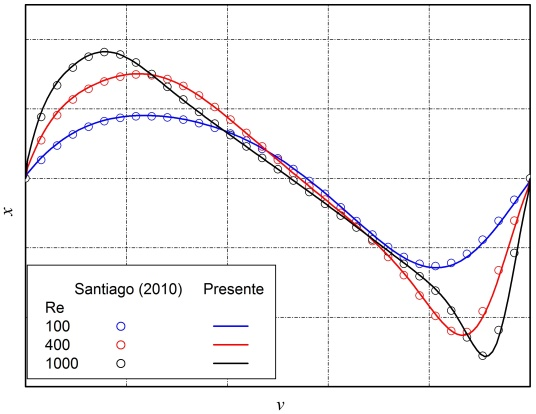
\includegraphics[width = \CaptionWidth]{grph-example}
% \SourceOrNote{Autoria Própria (2024)}
% \end{graph}

% Em computação, é muito comum a utilização de fluxogramas, para documentar, estudar, planejar, melhorar e comunicar processos complexos por meio de diagramas claros e fáceis de entender. Um fluxograma é um diagrama que descreve um processo, sistema ou algoritmo de computador. O \Cref{fcht:ex-algorithm} é um dos vários exemplos deste tipo de ilustração que pode ser gerado ou editado na ferramenta \textit{online} \href{http://www.lucidchart.com/}{Lucidchart}, entre outras.

% \begin{flowchart}[!htb]
% \centering
% \caption{Exemplo de fluxograma de algoritmo}%
% \label{fcht:ex-algorithm}
% 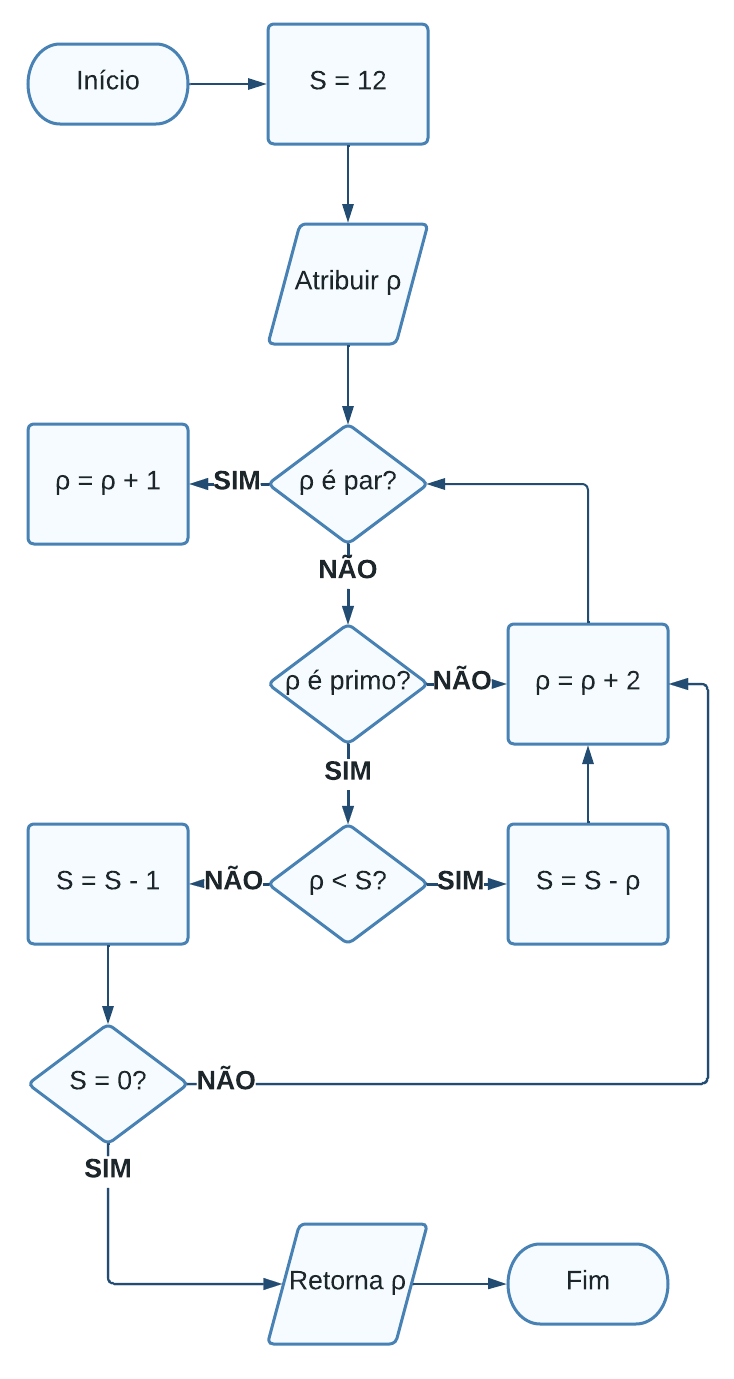
\includegraphics[scale=0.4]{fcht-ex-algorithm}
% \SourceOrNote{Autoria Própria (2024)}
% \end{flowchart}

% O LaTeX tem uma biblioteca específica para utilizar imagens no documento. O pacote graphicx habilita um ambiente chamado figure, que permite que você insira imagens de uma forma simples no texto. A \Cref{fig:example-image-duck} é um exemplo deste tipo de ilustração.

% \begin{figure}[!h]
% \centering
% \caption{Exemplo de figura}%
% \label{fig:example-image-duck}
% \includegraphics[scale=1.2]{example-image-duck}
% \SourceOrNote{Autoria Própria (2024)}
% \end{figure}

% Caso seja necessário, você ainda poderá inserir fotografias, por meio do ambiente \textit{photograph}, conforme ilustrado na \Cref{phot:pg-campus}.

% \begin{photograph}[!h]
% \centering
% \SetCaptionWidth{\ifbool{@LayoutA}{0.7}{0.72}\linewidth}
% \caption{Fachada da Fatec de Registro}%
% \label{phot:pg-campus}
% \savebox0{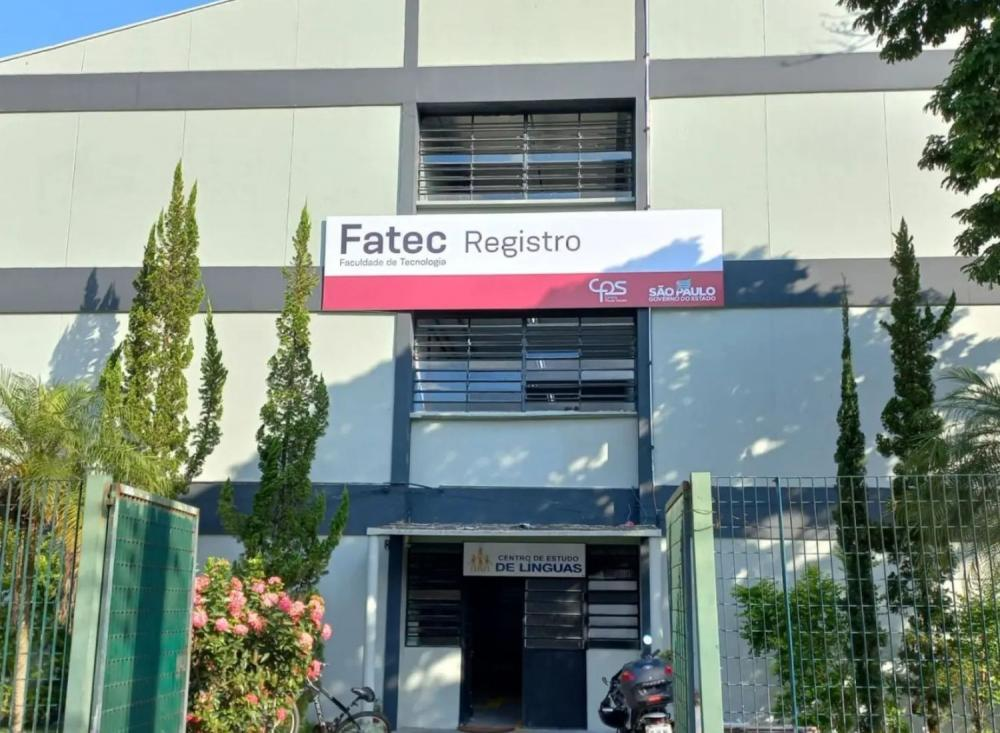
\includegraphics[width = \CaptionWidth]{Illustrations/fachada-fatec.jpg}}
% \usebox0%
% \SourceOrNote{Autoria Própria (2024)}
% \end{photograph}

% Outro elemento visual bastante utilizado na seção de Resultados são as tabelas, pois elas fornecem uma estrutura visualmente organizada para apresentar dados, tornando a leitura e a compreensão do conteúdo mais fácil para o leitor. As células, linhas e colunas ajudam a alinhar informações de maneira sistemática.

% Para conjuntos de dados comparativos, as tabelas são particularmente úteis. Elas possibilitam a disposição lado a lado de informações relacionadas, facilitando a comparação direta entre diferentes elementos.

% Tabelas e quadros devem estar centralizados e conter apenas dados imprescindíveis, evitando-se que sejam muito extensos, não repetindo dados já inseridos no texto, ou vice-versa. O formato de tabela pode ser observado na \Cref{tab:example}.

% \begin{table}[!htb]
% \centering
% \SetCaptionWidth{0.5\linewidth}
% \caption{Exemplo de tabela}%
% \label{tab:example}
% \begin{tabularx}{\CaptionWidth}{@{}XY@{}}
% \toprule%
% \rowcolor{TableColor}
% \multicolumn{1}{Y}{\textcolor{white}{Idade}}           &
% \multicolumn{1}{Y}{\textcolor{white}{Percentual (\%)}} \\
% \midrule%
% Até 20 anos     & 0  \\
% De 21 a 30 anos & 10 \\
% De 31 a 40 anos & 20 \\
% De 41 a 50 anos & 30 \\
% \bottomrule%
% \end{tabularx}
% \SourceOrNote{Adaptada de \textcite{Beltrano2021}}
% \end{table}

% No caso de quadros, deve ser seguida a estrutura demonstrada no \Cref{tfrm:typography}.
% Caso os dados sejam inéditos e provenientes de uma pesquisa realizada pelos próprios autores do trabalho, essa especificação deve constar na fonte com o ano da pesquisa de campo.
% Nesse caso, a fonte deve ser: Autoria Própria (2024).

% \begin{tabframed}[!htb]
% \centering
% \caption{Tipografia das seções}%
% \label{tfrm:typography}
% \begin{tabularx}{\linewidth}{?{}p{20mm}|X|p{45mm}?{}}%% CHKTEX 44
% \toprule%
% \rowcolor{TableColor}
% \multicolumn{1}{?{}c|}{\textcolor{white}{Seção}}   &
% \multicolumn{1}{c|}{\textcolor{white}{Tipografia}} &
% \multicolumn{1}{c?{}}{\textcolor{white}{Exemplo}}  \\
% \midrule%
% Primária                     &
% Letras maiúsculas em negrito &
% \textbf{1 SEÇÃO PRIMÁRIA}    \\
% \midrule%
% Secundária                    &
% Letras maiúsculas sem negrito &
% 1.1 SEÇÃO SECUNDÁRIA          \\
% \midrule%
% Terciária                                                             &
% Letra inicial de todas as palavras em maiúscula, sem negrito &
% 1.1.1 Seção Terciária                                                 \\
% \midrule%
% Quaternária                                                          &
% Letra inicial da primeira palavra em maiúscula, sem negrito &
% 1.1.1.1 Seção quaternária                                            \\
% \midrule%
% Quinária                                                                          &
% Letra inicial da primeira palavra em maiúscula, sem negrito e em itálico &
% \textit{1.1.1.1.1 Seção quinária}                                                 \\
% \bottomrule%
% \end{tabularx}
% \SourceOrNote{Autoria Própria (2024)}
% \end{tabframed}

% Quadros e tabelas podem ser inseridos neste documento usando os ambientes \texttt{tabframed} e \texttt{table}, respectivamente, conforme exemplos no arquivo-fonte deste modelo. A geração ou edição desses elementos visuais pode ser realizada por meio de ferramentas \textit{online}, tais como: \href{http://www.tablesgenerator.com/}{Tables Generator} e \href{http://www.latex-tables.com/}{Latex Tables Editor}, entre outras.

% \subsection*{Equações}

% Equações podem ser inseridas neste documento usando o ambiente  \texttt{equation}, como ilustrado na \Cref{eq:u}.

% \begin{equation}%
% \label{eq:u}
% u = \beta \operatorname{sen} \left(\pi x\right) \frac{\left(e^{2x} - 1\right) \left(e^y - 1\right)}{\left(e^2 - 1\right) \left(e - 1\right)}
% \end{equation}

% Símbolos matemáticos (ou equações mais simples) podem ser inseridos ao longo do texto de um parágrafo usando o ambiente do Latex \texttt{math}. É possível ainda, a utilização de ferramentas onlines para a geração ou edição de equações, tais como: \href{http://formulasheet.com/}{Formula Sheet} e \href{http://www.tutorialspoint.com/latex_equation_editor.htm}{Latex Equation Editor}.

